\section{Estudi implementació \textit{mixer}}
S'ha considerat la possibilitat d'afegir un \textit{mixer} al turbofan calculat. El criteri de decisió és simple; si el \textit{mixer} millora l'empenta adimensinonal del rotor, i per tant redueix el consum específic, s'adoptarà. De no ser així, es mantindrà el motor sense \textit{mixer}. Per fer els càlculs necessaris s'ha creat la funció \textit{mixer.m}. Aquesta té com a objectiu calcular les condicions del fluid a la sortida del mixer en funció de l'entrada a aquest dels dos fluxos, el primari i el secundari.
\begin{figure}[H]
	\centering
	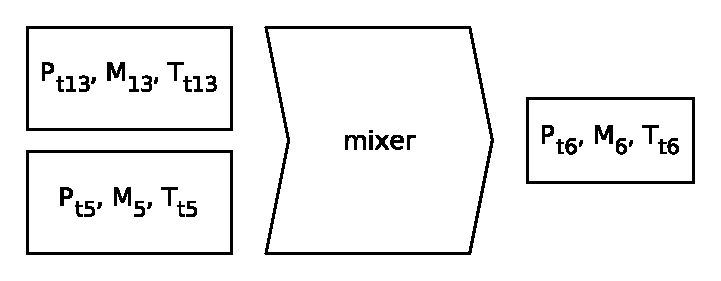
\includegraphics[scale=0.65]{./pics/mixer.eps}
	\caption{Treball del mixer}
\end{figure}
\noindent Pel que fa a les propietats termodinàmiques que depenen de la temperatura, es fa una mitjana ponderada per tal de trobar-les a la sortida. Per calcular altres valores necessaris com el Mach al flux secundari, s'imposa l'aproximació de que el flux al \textit{mixer} és laminar, de forma que les pèrdues siguin mínimes. Per fer això es prenen les següents hipòtesis:
\begin{itemize}
\item $M_5 = 1$
\item $P_5 = P_{13} = P_6$
\end{itemize}
Es tracta d'hipòtesis molt simplificatives que són poc realistes, ja que realment el \textit{mixer} serveix per barrejar el fluid del primari i del secundari i si el flux fos laminar no es produiria una barreja adecuada. 
Per últim, es fa us de l'equació de quantitat de moviment per trobar les condicions de sortida:
\begin{equation}
\label{ccm}
F_6 = F_5 + F_{13}
\end{equation}
On:
\begin{equation}
F = \dot{m}\sqrt{\frac{RT_t}{\gamma\phi}}
\end{equation}
\begin{equation}
\label{phi}
\phi = \Bigg[ \frac{M\sqrt{1+\frac{\gamma-1}{2}M^2}}{a+\gamma M^2}\Bigg]^2
\end{equation}
Amb la Eq.\ref{ccm} es pot acabar traient el $M_6$ que servirà també per trobar $P_{t6}$. Si s'observen les equacions amb atenció i es fa un estudi de la funció $\phi$ s'arriba a veure que aquesta té un màxim per Mach igual a 1 en el cual $\phi_6=0.208$. En el present cas d'estudi s'obté que pels paràmetres de disseny escollits $\phi_6=0.2314$, per la qual cosa el $M_6$ s'ha hagut de limitar a 1 evitant condicions supersòniques i evidenciant que el \textit{mixer} està ofegat.
A continuació es presenta la comparativa entre el motor sense \textit{mixer} i amb \textit{mixer}.
\begin{table}[H]
	\centering
	\begin{tabular}{lc}
		\toprule[3pt]
		\textbf{Paràmetre}&\textbf{Valor}\\
		\midrule[1pt]
		$\hat{F}$ & 6.29 \\
		$\hat{F}_{mixer}$ & 3.14 \\
		\bottomrule[2pt]
	\end{tabular}
	\label{C_opti2}
	\caption{Comparativa mixer}
\end{table}
\noindent Es pot concloure que el\textit{ mixer} perjudica al nostre motor doncs fa que l'empenta adimensional sigui més petita, el que voldria dir que el flux màssic necessari es major. Així doncs,\textbf{ no s'emprarà mixer.}